% This is samplepaper.tex, a sample chapter demonstrating the
% LLNCS macro package for Springer Computer Science proceedings;
% Version 2.20 of 2017/10/04
%
\documentclass[runningheads]{llncs}
% Imágenes
\usepackage{graphicx}
% Posición de las imágenes
\usepackage{float}
% Hipervínculos
\usepackage{hyperref}
% Tablas
\usepackage[table,xcdraw]{xcolor}
% Idioma y tildes
\usepackage[spanish]{babel}
\selectlanguage{spanish}
\usepackage[utf8]{inputenc}


\begin{document}

\title{PECL3. Cloud Computing.\\ Google Cloud, AWS y Azure}

\author{Pablo Acereda \and  David E.Craciunescu \and Ángel Martín,  Ángela Moreno y Laura Pérez Medeiro}

\institute{PECL3 \\ Ampliación de Programación Avanzada \\ Universidad Alcalá}
%
\maketitle              
% --------------------------------------------------------------------------------%
%------------------------------- D O C U M E N T O -------------------------------%
% --------------------------------------------------------------------------------%
\section{Servicios de IA y Machine learning en Cloud Computing}
\begin{abstract}
    En este apartado se detallará la información relativa a los servicios relativos a IA y maching learning haciendo uso de Azure o Amazon web services. Concretamente, hablaremos de los servicios cognitivos que usan. Estos servicios incorporan a las aplicaciones algoritmos inteligentes que permiten ver, oír, hablar, comprender e interpretar las necesidades de los usuarios con formas de comunicación naturales.
\end{abstract}

% ---------------------------- I N T R O D U C C I Ó N ---------------------------%
\subsection{Introducción}
    \subsubsection{Azure}
    Los recursos de Cognitive Service que encontramos en Azure se encuentran agrupados en cinco categorias: 
    \begin{itemize}
        \item Decision. Creación de aplicaciones que realicen recomendaciones útiles y eficientes para la toma de decisiones.
        \item Visión. Reconocimiento, identificación, subtitulado, indexado, moderación de imágenes, vídeos y contenido digital.
        \item Voz. Integración de capacidades de procesamiento de voz en aplicacioes.
        \item Lenguaje. Permite a las aplicaciones procesar lenguajes natural con scripts pre-construidos, evaluando el sentimiento y aprendiendo a reconocer qué es lo que los usuarios desean.
        \item Búsqueda. Permite añadir las APIs de Bing Search a las aplicaciones, aprovechando así la capacidad de combinar multitud de recursos (como otras páginas webs, vídeos, imágenes...) en una sola llamada API.
    \end{itemize}
    \subsubsection{Amazon Web Services}
    La estructura de las soluciones seguidas por Amazon Web Services es bastante diferente. Los apartados que se corresponderían con los de azure serían: aprendizaje automático y servicios multimedia.

% --------------------------  S E R V I C I O    A Z U R E  -------------------------- 

% ------------------------ P R U E B A    S E R V I C I O ------------------------ 
\subsection{Servicio de traducción}
Uno de los servicios que encontramos dentro de cada plataforma, es el servicio neural de traducción automática para la integración en aplicaciones, sitios web, herrramientas...
    \subsubsection{Azure Translator Text}
Este servicio con Azure nos permite:
\begin{enumerate}
    \item Traducir texto a más de 60 idiomas disponibles mediante la interfaz de REST abierta de Translator API.
    \item Detectar automáticamente el idioma, simplificando procesos de desarrollo y permitiendo enviar rápidamente la traducción
    \item Transcipción de diferentes alfabetos. Como la traducción de carácteres chinos al pinyin.
    \item Proporcionar contextos para traducciones alternativas, de esta manera los usuarios pueden elegir la traducción más adecuda para el contexto del recurso.
    \item Agregar soporte de traducción en línea o sin conexión a la aplicación.
    \item Crear sistemas de tradución personalizados.
\end{enumerate}{}
En cuanto al precio, encontramos desde una capa gratuita (la cual ofrece 2 millones de caracteres de cualquier combinación de traducción estándar y entrenamiento personalizado gratis por mes) a los 37.9448,503 euros al mes(donde se ofrece hasta 2500 millones de caracteres al mes, junto on una formación y un modelo de traducción personalizado hospedado por región al mes). Incluye soporte técino y administración de suscripciones de manera gratuita y garantiza una disponibilidad de 99.99\% para el nivel estándar.

\paragraph{Integración de Power BI con Text Analytics de Cognitive Services}
Utilizaremos el servicio de Text Analytics para extraer las frases más importantes, analizar las opiniones e identificar entidades conocidas como marcas. De esta forma se puede visualizar rápidamente lo que hablan los clientes acerca de nuestra marca o cómo se sienten al respecto.

Para ello, necesitaremos descargar Power BI Desktop (software utilizado anteriormente en la parte individual), una cuenta de Microsoft Azure donde crearemos un recurso para obtener los datos de una cuenta de Cognitive Service API que necesitaremos más tarde) y una base de datos con comentarios de los clientes o información a anlizar (usaremos una base de datos de ejemplo proporcionada por Azure).

La creación del recurso Cognitive Service puede realizarse mediante la subscripción a varios recursos o a un único servicio. Aquí se explicará la primera opción, ya que podremos utilizar estos datos para posteriores pruebas de otros servicios sin la necesidad de crear nuevos recursos. Para ello seleccionaremos ''crear recurso'' dentro de la página de inicio de nuestro Azure Portal, en el buscador pondremos ''Cognitive Service'' y seleccionaremos ''Crear''

\begin{figure}[H]

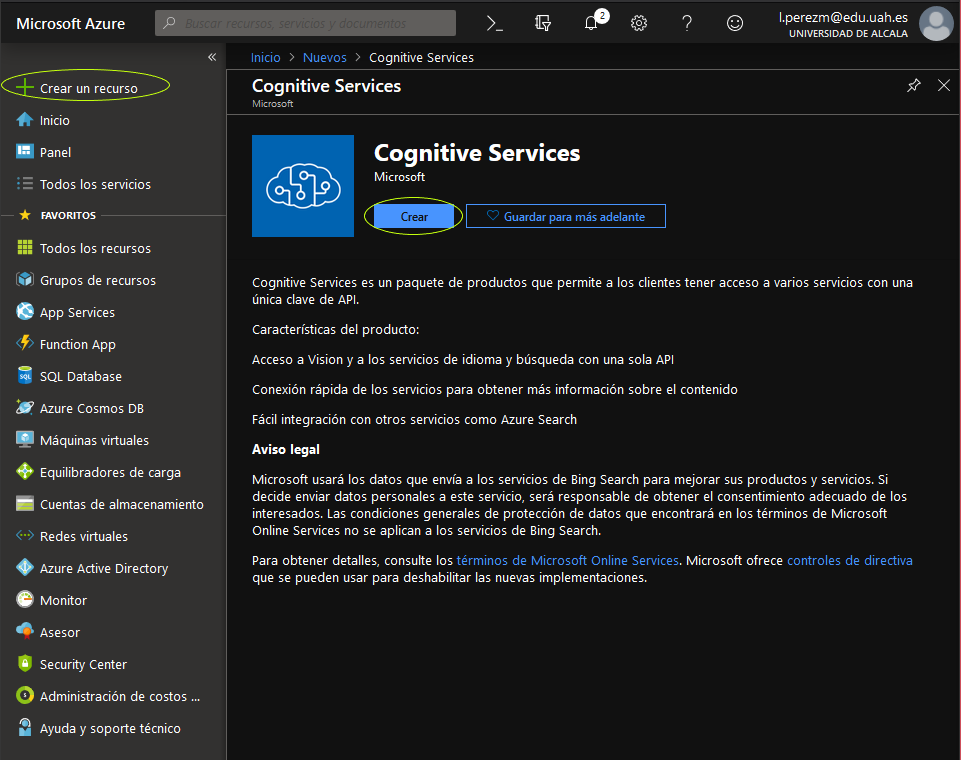
\includegraphics[scale = 0.25]{./IA/AZURE/crearRecursoCS.png}
\end{figure}
\newpage Completamos los campos de nuestro recurso:

\begin{figure}[H]
\centering
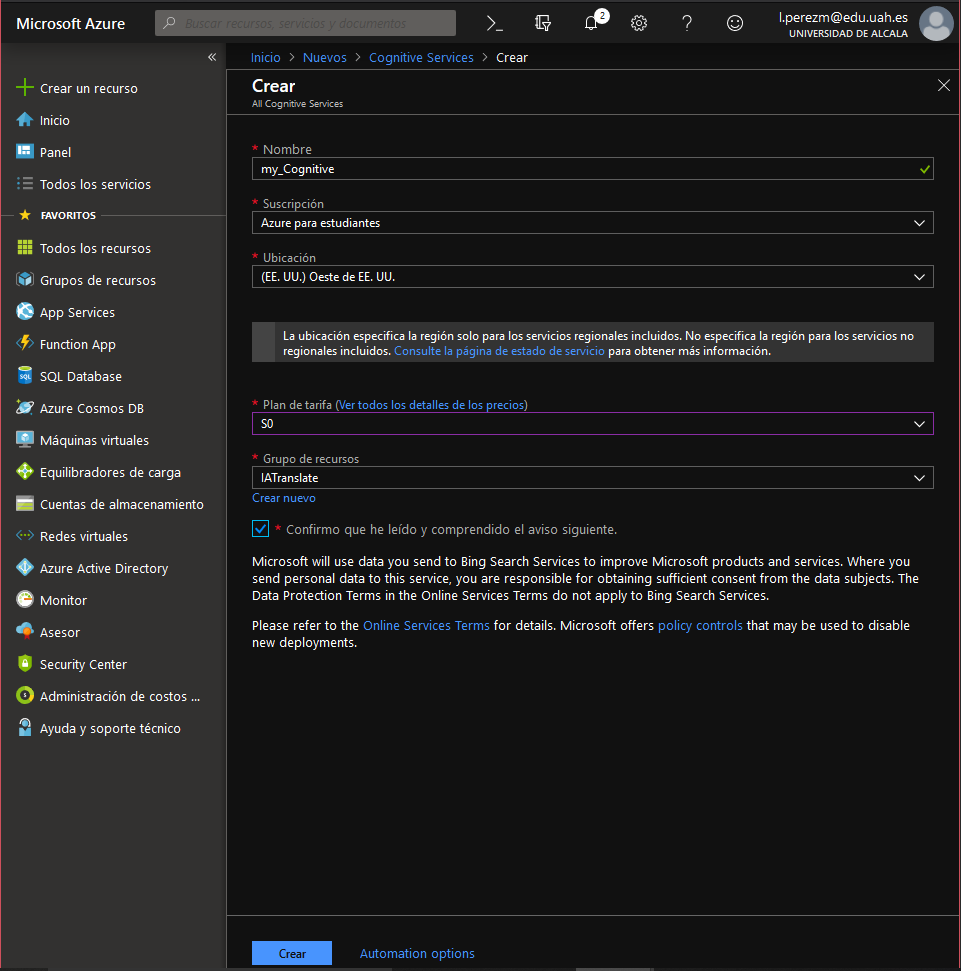
\includegraphics[scale = 0.25]{./IA/AZURE/confCognitive.PNG}
\caption{Ubicación es Oeste de EE.UU para evitar confusiones y problemas posteriores a la hora de especificar el URL del servicio}
\end{figure}


Para descargar los datos de ejemplo accedemos al enlace \url{ https://github.com/Kaiqb/KaiqbRepo0731190208/tree/master/CognitiveServices/TextAnalytics}, copiamos la información y la agregado a un archivo .csv. Una vez tenemos los datos, los importamos mediante la opción ''obtener datos'' > ''Texto/csv'' y la ubicación donde se haye el archivo con los datos.

\begin{figure}[H]

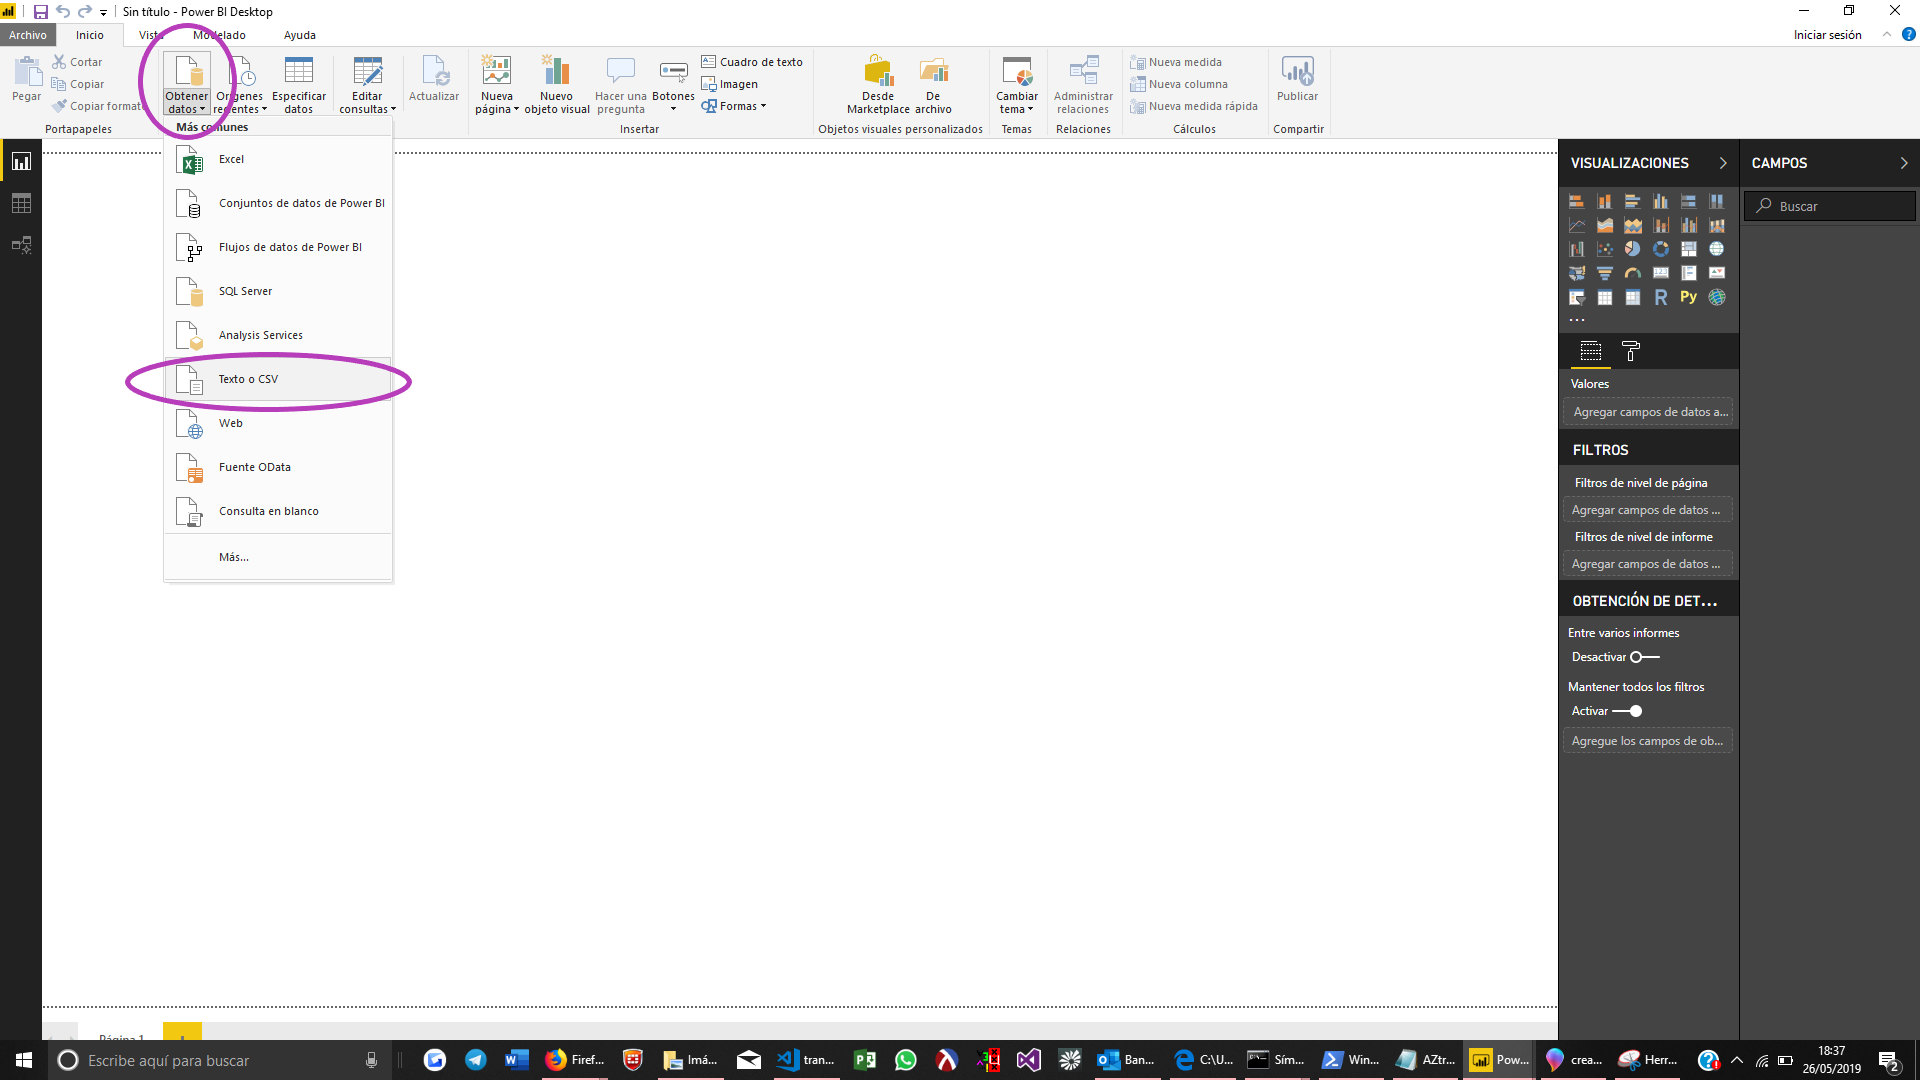
\includegraphics[scale=0.25]{./IA/AZURE/loadData.png}
\end{figure}

Una vez están los datos en Power BI, seleccionamos \textit{Inicio} / \textit{Datos Externos}/ \textit{Editar consultas}.

Dentro de la nueva pestaña abierta seleccionamos las columnas "subject" y "comment". A continuación seleccionamos \textit{Transformar} / \textit{Columnas de texto} / \textit{Combinar Columnas}

\begin{figure}[H]
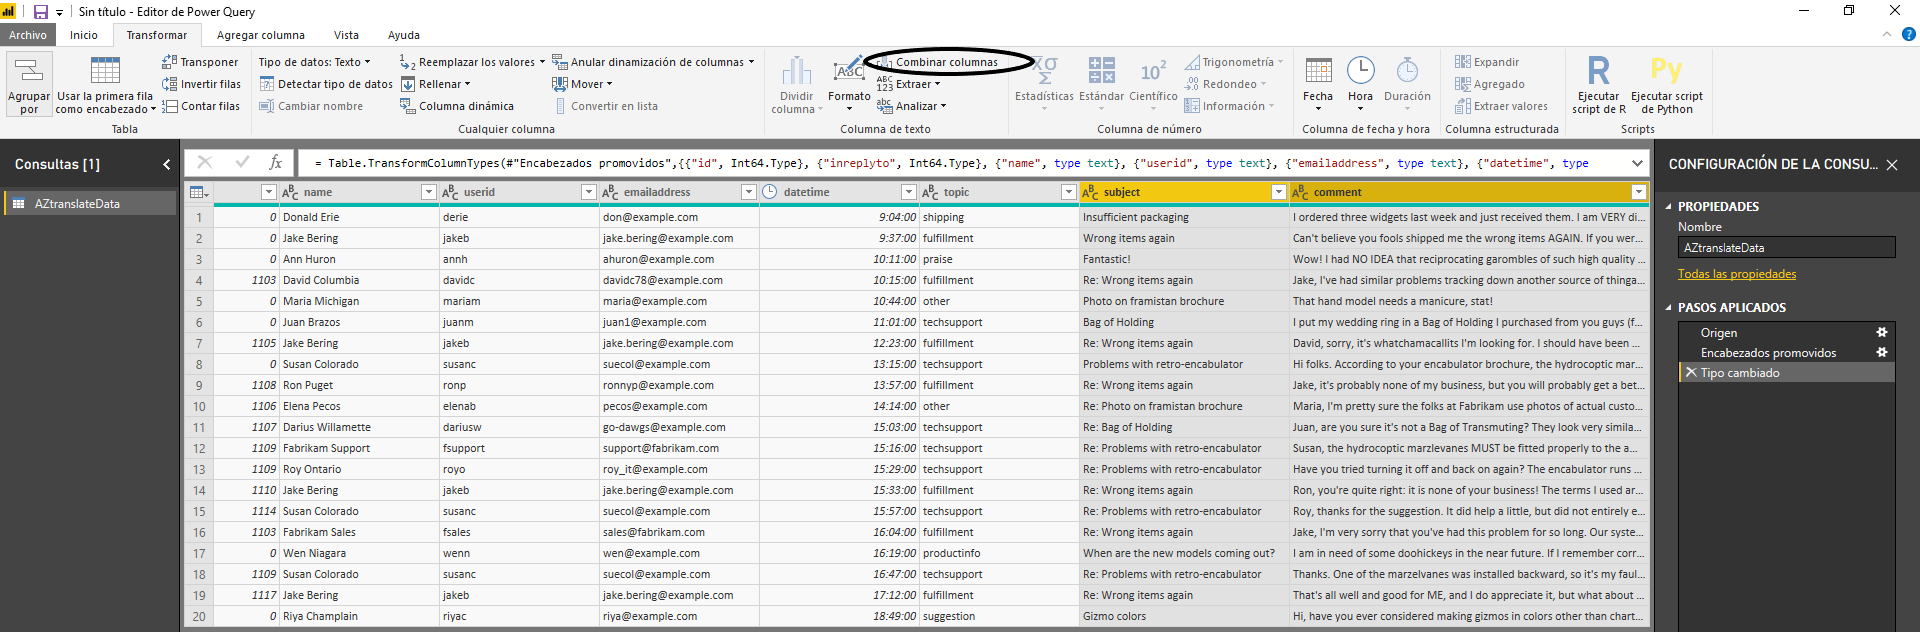
\includegraphics[scale=0.25]{./IA/AZURE/combinarColumnas.png}
\end{figure}

En el cuadro de diálogo seleccionamos 

\begin{figure}[H]
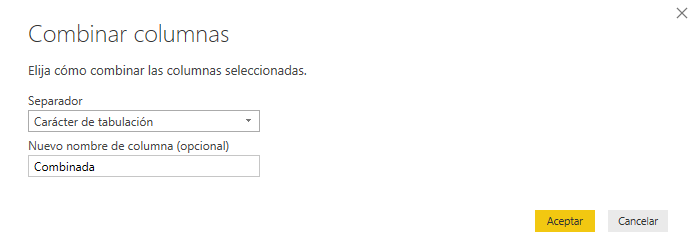
\includegraphics[scale=0.25]{./IA/AZURE/comCol.png}
\end{figure}

Sin salir de la ventada del Editor de consultas seleccionamos \textit{Inicio} / \textit{Nueva Consulta} y dentro del menú desplegable \textit{Nuevo origen}/ \textit{consulta en blanco}. Aparecerá una nueva consulta, a la cual se le cambiará el nombre si se desea.
Ahora, seleccionamos \textit{Inicio} / \textit{Consulta} / \textit{Editor Avanzado}, eliminaremos el código que aparece y lo sustituiremos por:
\small{
\begin{verbatim}

// Returns key phrases from the text in a comma-separated list
(text) => let
    apikey      = "YOUR_API_KEY_HERE",
    endpoint    = "https://westus.api.cognitive.microsoft.com/text/analytics/v2.1/keyPhrases",
    jsontext    = Text.FromBinary(Json.FromValue(Text.Start(Text.Trim(text), 5000))),
    jsonbody    = "{ documents: [ { language: ""en"", id: ""0"", text: " & jsontext & " } ] }",
    bytesbody   = Text.ToBinary(jsonbody),
    headers     = [#"Ocp-Apim-Subscription-Key" = apikey],
    bytesresp   = Web.Contents(endpoint, [Headers=headers, Content=bytesbody]),
    jsonresp    = Json.Document(bytesresp),
    keyphrases  = Text.Lower(Text.Combine(jsonresp[documents]{0}[keyPhrases], ", "))
in  keyphrases
}
\end{verbatim}
}
La variable apikey deberá contener la calve de acceso de Text Analytics y end point será la url de nuestro recurso: 
\begin{figure}[H]
\centering
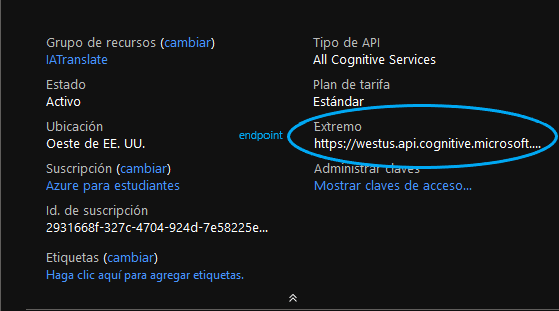
\includegraphics[scale=0.25]{./IA/AZURE/infoCog.png}
\end{figure}
\begin{figure}[H]
\centering
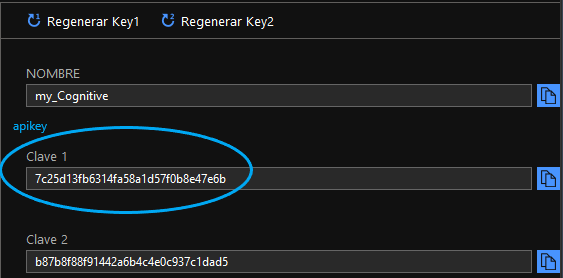
\includegraphics[scale=0.25]{./IA/AZURE/keyconf.png}
\end{figure}

En Power BI seleccionamos \textit{Agregar Columna} / \textit{General} / \textit{Invocar función personalizada}, aparecerá un cuadro de diálogo en donde pondremos un \textbf{nuevo nombre de columna}, seleccionaremos como \textbf{Consulta de función} el nombre que le hayamos dado a la consulta, y como texto elegiremos Combinada.

Una vez está todo listo, crearemos nuestra nube de palabras. Esta nube se podría crear directamente desde power BI pero actualmente, no se cuentan con los permisos por darte de la organización para ello. Por eso haremos uso de la columna generada por nuestra función y el enlace \url{https://www.jasondavies.com/wordcloud/}, teniendo como resultado: 

\begin{figure}[H]
\centering
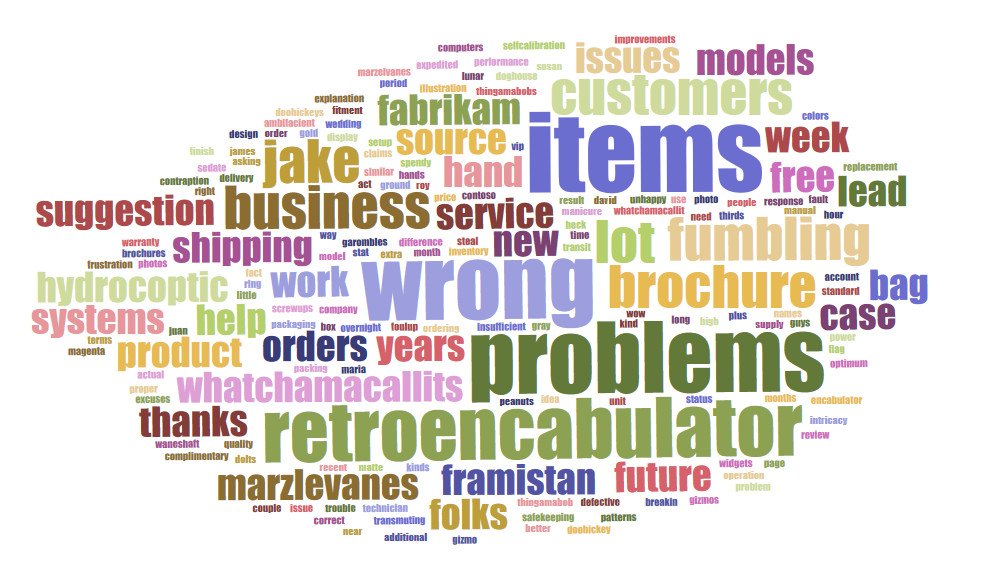
\includegraphics[scale=0.5]{./IA/AZURE/wordcloud.png}
\end{figure}
Otra función que podemos aplicar en Power BI Desktop es en análisis de sentimiento, la cual decolvería una puntuación que indicara el grado de positivo o negativo del sentimiento extresado para el texto, Para esto se usaría el siguiente fragmento de cógigo:

\small{
\begin{verbatim}

// Returns the sentiment score of the text, from 0.0 (least favorable) to 1.0 (most favorable)
(text) => let
    apikey      = "YOUR_API_KEY_HERE",
    endpoint    = "https://westus.api.cognitive.microsoft.com/text/analytics/v2.1/sentiment",
    jsontext    = Text.FromBinary(Json.FromValue(Text.Start(Text.Trim(text), 5000))),
    jsonbody    = "{ documents: [ { language: ""en"", id: ""0"", text: " & jsontext & " } ] }",
    bytesbody   = Text.ToBinary(jsonbody),
    headers     = [#"Ocp-Apim-Subscription-Key" = apikey],
    bytesresp   = Web.Contents(endpoint, [Headers=headers, Content=bytesbody]),
    jsonresp    = Json.Document(bytesresp),
    sentiment   = jsonresp[documents]{0}[score]
in  sentiment
\end{verbatim}
}
    \subsubsection{Amazon Translate}
El servicio de Amazon Translate usa técnicas de aprendizaje profundo, con la finalidad de ofrecer traducciones más precisas y fluidas que las obtenidas con traductores estadísticos tradicionales y basados en reglas.
Con este servicio, amazon nos ofrece un alto grado de calidad, garantiza un grado alto de facilidad con la escalidbilidad del servicio, ofrece un servicio de traducción bajo demanda en tiempo real para contenido generado por usuarios o aplicaciones de comunicación. así como la seguridad de confidencialidad y no filtración de los documentos que pasen por este servicio.

Con este servicio, amazon quiere mejorar las experiencias multilingüe para los usuarios, ofrecer procesamiento de datos en varios idiomas, mejorar las comunicaciones internas y externas de la empresa así como la posibilidad de tener una traducción rápida y fiable de grandes volúmenes de contenido almacenado en bases de datos u objetos.

Encontramos dos tarifas para este servicio:
\begin{itemize}
    \item Capa gratuita: los primeros 2 millones de caracteress de cada ciclo mensual son gratuitos durante el primer año.
    \item 15\$ por millon de caracteres
El servicio es de pago por uso, no hay tarifa ninguna por mantenimiento ni instalación.

\end{itemize} 
Los idiomas que encontramos disponibles son: chino, indonesio, japonés, coreano, malayo, danés, neerlandés, alemán, inglés, noruego, sueco, francés, italiano, españolm portugués, árabe, hebreo, hindi, persa, finés y turco. Aunque hay algunos idiomas que pueden no estar disponibles según en la región AWS GovCloud que nos encontremos. Otra restricción que encontramos es la incompatibilidad de pares entre algunos idiomas como de coreano a hebreo.


Para tener un mayor conocimiento de Amazon Translate, se consulta la documentación de este y en ella se especifica que tenemos que crear un usuario IAM que sea el administrador del recurso, sin embargo, al comenzar los pasos para realizarlo se encuentran que no se poseen los requisitos necesarios para llevar a cabo esta acción:

\begin{figure}[H]
\centering
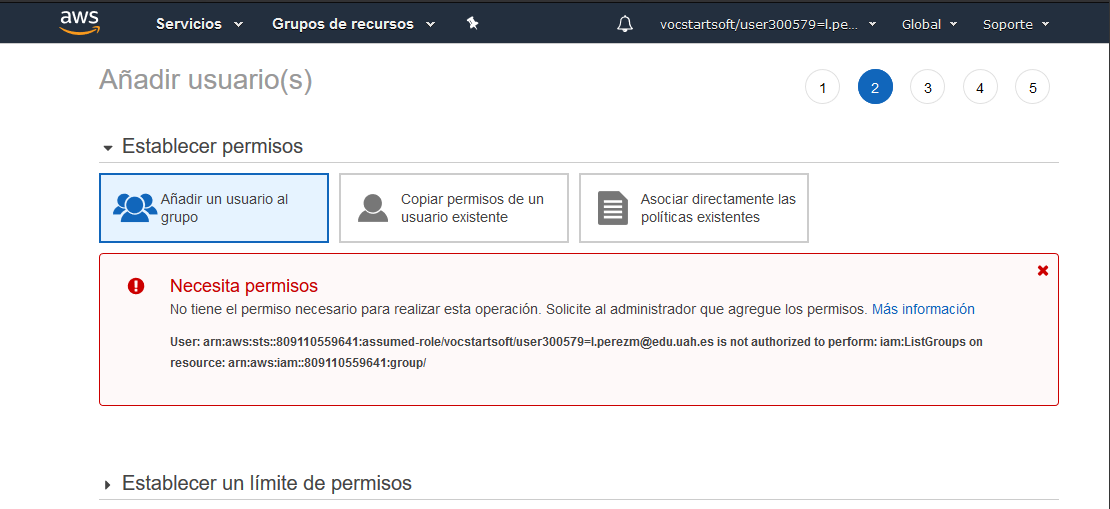
\includegraphics[scale=0.5]{./IA/AWS/denyedpermissionAWS.png}
\end{figure}

El siguiente paso consiste en configurar la AWS Command Line Interface, para  ello necesitaremos tener la version 2.6.5+ o 3.3+ de python y ejecutar en el terminal:

\begin{figure}[H]
\centering
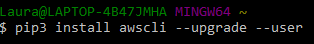
\includegraphics[scale=0.5]{./IA/AWS/pipAWS.png}
\end{figure}

Despues, tendremos que añadir a PATH la ruta del archivo ejecutable, y haciendo uso del comando "aws --version" comprobar que la instalación se ha producido exitosamente. Sin embargo, el siguiente paso a realizar sería la configuración de AWS CLI con el usuario Administrador que deberíamos haber creado.

Con AWS CLI podemos traducir hasta 5000 caracteres y obtendríamos como salida un archivo JSON como resultado de la traducción.

El comando para la shell sería:
aws translate translate-text \
            --region region \
            --source-language-code "en" \
            --target-language-code "es" \
            --text "hello, world " 
y obtendríamos el archivo:
\{
    "TargetLanguageCode": "es",
    "Text": "Hola, mundo",
    "SourceLanguageCode": "en"
\}

Si en su lugar quisiéramos pasar un archivo JSON como entrada tendríamos que usar el comando:
aws translate translate-text \
            --region region \
            --cli-input-json file://translate.json > translated.json

Dentro de las opciones que tenemos de utilización de esta traducción no se encuentra la generación de una nube de información como en Azure, pero se encuentran funciones muy interesantes como el uso de Amazon Translate para traducir un canal de chat.

\paragraph{Traducción de un canal de chat con Amazon Translate}
\begin{enumerate}
    \item Instale y configure AWS SDK for JavaScript. Para ello necesitaremos npm (el administrador de paquetes de Node.js) o bower (administrador de paquetes para la red). \textbf{ATENCIÓN: No todos los servicios están disponibles de forma inmediata en el SDK.}
    \item Agregar en un archivo HTML del servidor web el código adjunto tras estos pasos.

    \item Cambiar el contenido de la etiquete \textit{<script>}
    por la ubicación donde se encuentra instalado el SDK para JavaScript
    \item Cambiar la reguión y el punto de enlace a la región donde se desea ejecutar las operaciones. \textbf{Se debe consultar el listado de regiones donde Amazon Polly es admitida, ya que no son todas, al igual que no todas son admitidas por Amazon Translate}
    \item Crear un usuario IAM con los permisos mínimos necesarios
    \item Proporcionar el ID de acceso y la clave secreta del usuario de IAM creado en el paso anterior
    \item Proporcione un nombre de usuario de Twitch y token de OAuth para la cuenta.
\end{enumerate}
    \small{
\begin{verbatim}
<!doctype html>
<html lang="en">
<head>
  <title>Amazon Translate</title>
  <meta charset="utf-8">
  <meta name="viewport" content="width=device-width, initial-scale=1, shrink-to-fit=no">

  <!-- Latest compiled and minified CSS for Bootstrap -->
  <link rel="stylesheet"
  href="https://maxcdn.bootstrapcdn.com/bootstrap/3.3.7/css/bootstrap.min.css"
  integrity="sha384-BVYiiSIFeK1dGmJRAkycuHAHRg32OmUcww7on3RYdg4Va+PmSTsz/K68vbdEjh4u" 
  crossorigin="anonymous">

   <!-- Custom CSS -->
   <style>
     .topHeader
     {
       background-color: #6441a4;
       padding: 10px;
       border-bottom: solid 1px #cacaca;
       color: white
     }

     .panelHeading
     {
       background-color: #6441a4 !important;
     }

     .panelBody
     {
      min-height: 450px;  max-height: 450px;overflow-y: scroll;
     }

     body{
        margin-left: 0px;
        margin-right: 0px;
        height: 100%;
      }
   </style>
</head>
<body>
  <div class="container-fluid">
    <!--Top Header-->
    <div class="row topHeader">
      <div class="col-md-12">
          <h4>Amazon Translate - Artificial Intelligence on AWS
          - Powerful machine learning for all Developers 
          and Data Scientists</h4>
      </div>
    </div>

    <!--Status Label-->
    <div class="row">
      <div class="col-md-12">
        <p class="bg-info">
        <div id="connecting-div"></div>
        </p>
      </div>
    </div>

    <div class="row" style="padding: 10px;">
      <div class="col-md-6">
          <div class="form-inline">
            <div class="form-group">
              <input 
              type="text" id="channel" class="form-control" 
              value="" placeholder="Channel"/>
            </div>
            <div class="form-group">
              <select id="sourceLanguage" class="form-control">
                  <option value="en">en</option>
                  <option value="ar">ar</option>
                  <option value="de" selected="selected">de</option>
                  <option value="es">es</option>
                  <option value="fr">fr</option>
                  <option value="pt">pt</option>
                  <option value="zh">zh</option>
                </select>
            </div>
            <div class="form-group">
              <select id="targetLanguage" class="form-control">
                <option value="en" selected="selected">en</option>
                <option value="ar">ar</option>
                <option value="de">de</option>
                <option value="es">es</option>
                <option value="fr">fr</option>
                <option value="pt">pt</option>
                <option value="zh">zh</option>
              </select>
            </div>
            <div class="form-group">
              <button type="button" class="form-control" id="btn-go" 
              onclick="connect()">Go</button>
              <button type="button" class="form-control" id="btn-stop"
              onclick="location.href='index.html';">Stop</button>
              <span id="status"></span>
            </div>
          </div>
        </div>
        <div class="col-md-6">
            <div class="form-inline">
              <div class="form-group">
                  <input type="checkbox" id="cbSpeak" value="Speak"> 
                  Speak Live Translation
                  <input type="text" id="follow" class="form-control" 
                  value="" placeholder="follow"/>
                </div>
            </div>
          </div>
      </div>

    <!--Chat Boxes-->
    <div class="row">
      <!--Live Chat-->
      <div class="col-md-6">
        <div class="panel panel-primary">
          <div class="panel-heading panelHeading">Live Chat</div>
            <div id="livechatc" class="panel-body panelBody">
              <div class="subscribe" id="livechat"></div>
          </div>
        </div>
      </div>
      <!--Live Chat-->
      <!--Translated Chat-->
      <div class="col-md-6">
        <div class="panel panel-primary">
          <div class="panel-heading panelHeading">Live Translation</div>
            <div id="livetranslationc" class="panel-body panelBody">
              <div class="imageDetected" id="livetranslation"></div>
          </div>
        </div>
      </div>
      <!--Translated Chat-->
    </div>

    <!--Send Message-->
    <div class="row">
        <div class="col-md-11">
            <input type="text" id="message" class="form-control"/>
        </div>
        <div class=" col-md-1">
          <button type="button" class="form-control btn btn-default" id="btn-send"
          onclick="sendMessage()">Send</button>
        </div>
    </div>
  </div>

   <!-- Latest compiled and minified JavaScript -->
   <!-- jQuery first, then Bootstrap JS -->
   <script src="https://code.jquery.com/jquery-3.2.1.slim.min.js"
   integrity="sha384-KJ3o2DKtIkvYIK3UENzmM7KCkRr/rE9/Qpg6aAZGJwFDMVNA/GpGFF93hXpG5KkN"
   crossorigin="anonymous"></script>
   <script src="https://maxcdn.bootstrapcdn.com/bootstrap/3.3.7/js/bootstrap.min.js"
   integrity="sha384-Tc5IQib027qvyjSMfHjOMaLkfuWVxZxUPnCJA7l2mCWNIpG9mGCD8wGNIcPD7Txa"
   crossorigin="anonymous"></script>

   <script src="aws-js-sdk/dist/aws-sdk-all.js"></script>
   <script src="http://cdn.tmijs.org/js/1.2.1/tmi.min.js"
   integrity="sha384-eE0n7sm1W7DOUI2Xh5I4qSpZTe6hupAO0ovLfqEy0yVJtGRBNfssdmjbJhEYm6Bw"
   crossorigin="anonymous"></script>
   <script>
     cred = {
          twitchUsername: "Twitch user name",
          twitchOAuthToken: "Twitch OAuth token",
          awsAccessKeyId: "access key",
          awsSecretAccessKey: "secret key"
     };

     AWS.config.region = 'region';
     ep = new AWS.Endpoint('endpoint');

     AWS.config.credentials = new AWS.Credentials(cred.awsAccessKeyId, cred.awsSecretAccessKey);
     window.translator = new AWS.Translate({endpoint: ep, region: AWS.config.region});

     /**************************Init and Connect to Chat****************************/
     function connect(){
       init();

       //Twitch Client
       var options = {
           options: {
             debug: false
           },
           connection: {
             cluster: "aws",
             reconnect: true
           },
           identity: {
             username: cred.twitchUsername,
             password: cred.twitchOAuthToken
           },
           channels: [con.channel]
       };

       window.client = tmi.client(options);

       window.client.connect();

       //Attached Handlers
       window.client.on("chat", onChat);
       window.client.on("connecting", onConnecting);
       window.client.on("connected", onConnected);

       //Disable UI Elements
       document.getElementById("sourceLanguage").disabled = true;
       document.getElementById("targetLanguage").disabled = true;
       document.getElementById("channel").disabled = true;
       document.getElementById("btn-go").disabled = true;
     }

     function init(){
       //Get UI Controls
       var lc = document.getElementById("livechat");
       var lt = document.getElementById("livetranslation")
       var lcc = document.getElementById("livechatc");
       var ltc = document.getElementById("livetranslationc")
       var cbspeak = document.getElementById("cbSpeak")
       var follow = document.getElementById("follow");
       var sendMessage = document.getElementById("message");

       //Cache values
       con = {
         channel: document.getElementById("channel").value,
         sourceLanguage: document.getElementById("sourceLanguage").value,
         targetLanguage: document.getElementById("targetLanguage").value,
         liveChatUI: lc,
         liveTranslationUI: lt,
         liveChatUIContainer: lcc,
         liveTranslationUIContainer: ltc,
         cbSpeak: cbspeak,
         follow: follow,
         sendMessage: sendMessage
       }

         lc.innerHTML = '';
         lt.innerHTML = '';

         //Speaker
        var voiceId = "Joanna";
        if(con.targetLanguage == "en")
           voiceId = "Joanna";
        else if(con.targetLanguage == "de")
             voiceId = "Marlene";
        else if(con.targetLanguage == "es")
            voiceId = "Conchita";
        else if(con.targetLanguage == "fr")
           voiceId = "Celine";
        else if(con.targetLanguage == "pt")
           voiceId = "Ines";
        else
           voiceId = "Joanna";
         window.audioPlayer = AudioPlayer(voiceId);
     }
     /**************************Init and Connect to Chat****************************/

     /**************************Receive and Translate Chat****************************/
     function onChat (channel, userstate, message, self) {
         // Don't listen to my own messages..
         if (self) return;

         //Translate
         if (message) {
           var username = userstate['username'];

           var params = {
               Text: message,
               SourceLanguageCode: con.sourceLanguage,
               TargetLanguageCode:  con.targetLanguage
           };

           window.translator.translateText(params, 
           function onIncomingMessageTranslate(err, data) {
              if (err) {
                 console.log("Error calling Translate. " + err.message + err.stack);
             }
              if (data) {
                  console.log("M: " + message);
                  console.log("T: " + data.TranslatedText);

                  //Print original message in chat UI
                  con.liveChatUI.innerHTML += '<strong>' + username + 
                  '</strong>: ' +  message + '<br>';

                  //Print translation in translation UI
                  con.liveTranslationUI.innerHTML += '<strong>' 
                  + username + '</strong>: ' +
                  data.TranslatedText + '<br>';

                  //If speak translation in enabled, speak translated message
                  if(con.cbSpeak.checked){
                    if(con.follow.value == "" || username == con.follow.value)
                      audioPlayer.Speak(username + " says " + data.TranslatedText);
                  }

                  //Scroll chat and translated UI to bottom to keep focus on latest messages
                  con.liveChatUIContainer.scrollTop = 
                  con.liveChatUIContainer.scrollHeight;
                  con.liveTranslationUIContainer.scrollTop = 
                  con.liveTranslationUIContainer.scrollHeight;
                }
           });
         }
     }
     /**************************Receive and Translate Chat****************************/

     /**************************Client Connecting****************************/
     function onConnecting (address, port) {
         document.getElementById("status").innerHTML = " [ Connecting...]"
     }

     function onConnected (address, port) {
         document.getElementById("status").innerHTML = " [ Connected ]"
         window.audioPlayer.Speak("Connected to channel " + con.channel +
         ". You should now be getting live
         chat messages.");
     }
     /**************************Client Connecting****************************/

     /**************************Send Message****************************/
     function sendMessage(){
          if(con.sendMessage.value){
            message = con.sendMessage.value;
            var params = {
                Text: con.sendMessage.value,
                SourceLanguageCode: con.targetLanguage,
                TargetLanguageCode:  con.sourceLanguage
            };

            window.translator.translateText(params, function onSendMessageTranslate(err, data) {
                  if (err) {
                     console.log("Error calling Translate. " + err.message + err.stack);
                  }
                  if (data) {
                      console.log("M: " + message);
                      console.log("T: " + data.TranslatedText);

                      //Send message to chat
                      window.client.action(con.channel, data.TranslatedText);

                      //Clear send message UI
                      con.sendMessage.value = "";

                      //Print original message in Translated UI
                      con.liveTranslationUI.innerHTML +=
                      '<strong> ME: </strong>: ' +  message + '<br>';

                      //Print translated message in Chat UI
                      con.liveChatUI.innerHTML += 
                      '<strong> ME: </strong>: ' + data.TranslatedText + '<br>';

                      //Scroll chat and translated UI to bottom to keep focus on latest messages
                      con.liveChatUIContainer.scrollTop = 
                      con.liveChatUIContainer.scrollHeight;
                      con.liveTranslationUIContainer.scrollTop = 
                      con.liveTranslationUIContainer.scrollHeight;
                  }
            });
          }
     }
     /**************************Send Message****************************/

     /**************************Audio player****************************/
     function AudioPlayer(voiceId) {
         var audioPlayer = document.createElement('audio');
         audioPlayer.setAttribute("id", "audioPlayer");
         document.body.appendChild(audioPlayer);

         var isSpeaking = false;

         var speaker = {
             self: this,
             playlist:[],

             Speak: function (text) {
                 //If currently speaking a message, add new message to the playlist
                 if (isSpeaking) {
                     this.playlist.push(text);
                 } else {
                     speakTextMessage(text).then(speakNextTextMessage)
                 }
             }
         }

         // Speak text message
         function speakTextMessage(text) {
             return new Promise(function (resolve, reject) {
                 isSpeaking = true;
                 getAudioStream(text).then(playAudioStream).then(resolve);
             });
         }

         // Speak next message in the list
         function speakNextTextMessage() {
             var pl = speaker.playlist;
             if (pl.length > 0) {
                 var txt = pl[0];
                 pl.splice(0, 1);
                 speakTextMessage(txt).then(speakNextTextMessage);
             }
         }

         // Get synthesized speech from Amazon polly
         function getAudioStream(textMessage) {
             return new Promise(function (resolve, reject) {
                 var polly = new AWS.Polly();
                 var params = {
                     OutputFormat: 'mp3',
                     Text: textMessage,
                     VoiceId: voiceId
                 }
                 polly.synthesizeSpeech(params, function (err, data) {
                     if (err)
                         reject(err);
                     else
                         resolve(data.AudioStream);
                 });
             });
         }

         // Play audio stream
         function playAudioStream(audioStream) {
             return new Promise(function (resolve, reject) {
                 var uInt8Array = new Uint8Array(audioStream);
                 var arrayBuffer = uInt8Array.buffer;
                 var blob = new Blob([arrayBuffer]);

                 var url = URL.createObjectURL(blob);
                 audioPlayer.src = url;
                 audioPlayer.addEventListener("ended", function () {
                     isSpeaking = false;
                     resolve();
                 });
                 audioPlayer.play();
             });
         }

         return speaker;
     }
     /**************************Audio player****************************/
   </script>
</body>
</html>

\end{verbatim}
}

% ---------------------------- C O N C L U S I O N E S  -----------------------------% 
\subsection{Conclusiones}
Dentro del campo de la inteligencia artificial y machine learning encontramos un mayor número de servicios ofertados por Azure, además de que todos ellos cuentan con un período de prueba de 7 días para conocer su funcionamiento. Además, Azure cuenta con muchas menos restricciones de las que podemos encontrar en AWS (en nuestro caso, con el servicio de traducciones no admite ciertos pares de idiomas a la hora de realizar la traducción, además de contar con un menor número de idiomas disponibles).

En términos económicos, Azure cuenta con un mayor número de planes que se pueden adpatar mejor a las necesidades de la empresa. Además, la documentación de Azure es tiene mayor grado de detalle, con una clara estructura de los pasos y únicamente redireccionándote a aquellos links de información adicional verdaderamente importantes, de lo contrario, los pasos necesarios son explicados (aunque si se quiere tener mayor detalle de ellos sigue existiendo la opción de clickar en el hipervínculo).

El uso de la interfaz de Azure es más intuitivo que el que encontramos dentro de Amazon Web Services, hecho que facilita enormemente la labor de implementación de los servicios y su testeo.

A modo resumen, se adjunta a continuación los diferentes servicios de cada apartado que encontramos en cada una de las nubes:

%----------- tablas de resumen/comparativa de los distintos servicios de IA ----------- 
\begin{table}[]
\begin{tabular}{|l|l|}
\hline
\multicolumn{2}{|l|}{{\color[HTML]{333333} MACHINE LEARNING}} \\ \hline
AWS & AZURE \\ \hline
SageMaker & \begin{tabular}[c]{@{}l@{}}Azure Machine\\ Learnig Studio\\ \\ Servicio Azure\\ Learning\end{tabular} \\ \hline
\end{tabular}
\end{table}

\begin{table}[]
\begin{tabular}{|l|l|}
\hline
\multicolumn{2}{|l|}{{\color[HTML]{333333} Servicios de voz y conversación}} \\ \hline
AWS & AZURE \\ \hline
\begin{tabular}[c]{@{}l@{}}Amazon Lex\\ Amazon Polly\end{tabular} & \begin{tabular}[c]{@{}l@{}}Bing Speech API\\ Speaker Recognition API\end{tabular} \\ \hline
\end{tabular}
\end{table}

\begin{table}[]
\begin{tabular}{|l|l|}
\hline
\multicolumn{2}{|c|}{{\color[HTML]{333333} Vision}} \\ \hline
AWS & AZURE \\ \hline
Amazon Rekognition & \begin{tabular}[c]{@{}l@{}}Computer Vision\\ Face API\\ Emotions API\end{tabular} \\ \hline
\end{tabular}
\end{table}

\begin{table}[]
\begin{tabular}{|l|l|}
\hline
\multicolumn{2}{|c|}{{\color[HTML]{333333} Lenguaje y Traducción}} \\ \hline
AWS & AZURE \\ \hline
\begin{tabular}[c]{@{}l@{}}Amazon Comprenhed\\ \\ \\ \\ Amazon Translate\end{tabular} & \begin{tabular}[c]{@{}l@{}}LUIS (Languaje Understanding \\ Intelligent Service)\\ \\ Translator Text\end{tabular} \\ \hline
\end{tabular}
\end{table}

\begin{table}[]
\begin{tabular}{|l|l|}
\hline
\multicolumn{2}{|c|}{{\color[HTML]{333333} Video}} \\ \hline
AWS & AZURE \\ \hline
\begin{tabular}[c]{@{}l@{}}Amazon Rekognition\\ Video\end{tabular} & Video API \\ \hline
\end{tabular}
\end{table}

\begin{table}[]
\begin{tabular}{|l|l|}
\hline
\multicolumn{2}{|c|}{{\color[HTML]{333333} Bots (Asistentes personales)}} \\ \hline
AWS & AZURE \\ \hline
Alexa Skils Kit & \begin{tabular}[c]{@{}l@{}}Azure AI\\ Bot Framework\end{tabular} \\ \hline
\end{tabular}
\end{table}


\paragraph{NOTAS:} Se comezó este apartado estudiando las posibilidades que ofrecia Azure en Computer Vision, pero su implemtación producía errores cuya solución es desconocida por el momento.

\begin{thebibliography}{8}


\bibitem{info-AmazonTranslate}
\textit{Documentación de AWS sobre Amazon translate} [en línea] \url{https://us-east-2.console.aws.amazon.com/translate/home?region=us-east-2#welcome}

\bibitem{info-AmazonTranslate}
\textit{Traducción de texto dentro de Cloud} [en línea] \url{https://aws.amazon.com/es/getting-started/tutorials/translate-text-between-languages-cloud/}

\bibitem{guia-desarrollo}
\textit{Amazon Translate y sus restricciones} [en línea] \url{https://docs.aws.amazon.com/es_es/translate/latest/dg/what-is.html}

\bibitem{creacion-traductor}
\textit{Amazon Translate y sus restricciones} [en línea] \url{https://aws.amazon.com/es/blogs/machine-learning/building-your-personal-translator-with-amazon-translate-and-amazon-polly/}

\bibitem{conf-AWSPowerShell}
\textit{Amazon Translate y sus restricciones} [en línea] \url{https://docs.aws.amazon.com/es_es/powershell/latest/userguide/pstools-getting-set-up-windows.html}

\bibitem{info-cogServices}
\textit{Explore Cognitive Services} [en línea] \url{https://azure.microsoft.com/es-es/services/cognitive-services/}

\bibitem{info-translatorAPI}
\textit{¿Qué es Translator Text API?} [en línea] \url{https://docs.microsoft.com/es-es/azure/cognitive-services/translator/translator-info-overview}

\bibitem{quickstart}
\textit{Inicio rápido: Compilación, implementación y uso de un modelo personalizado para la traducción} [en línea] \url{https://docs.microsoft.com/es-es/azure/cognitive-services/translator/custom-translator/quickstart-build-deploy-custom-model}

\bibitem{sub-translator}
\textit{Cómo suscribirse a Translator Text API} [en línea] \url{https://docs.microsoft.com/es-es/azure/cognitive-services/translator/translator-text-how-to-signup#learn-test-and-get-support}

\bibitem{python-translator}
\textit{Inicio rápido: Uso de Python para llamar a Text Analytics de Cognitive Services} [en línea] \url{https://docs.microsoft.com/es-es/azure/cognitive-services/text-analytics/quickstarts/python}
\url{https://docs.microsoft.com/en-us/azure/cognitive-services/Text-Analytics/quickstarts/python}
\url{https://docs.microsoft.com/en-us/azure/cognitive-services/translator/reference/v3-0-reference}

\end{thebibliography}

\end{document}
